\documentclass{article}
\usepackage{CJKutf8}
\usepackage{multirow}
\usepackage{listings}
\usepackage{graphicx}
\usepackage{amsmath}
\usepackage{subfigure}
\usepackage[colorlinks,linkcolor=red]{hyperref}
\begin{CJK}{UTF8}{gbsn}
\usepackage[framed,numbered,autolinebreaks]{mcode}
\begin{document}
\title{统计信号处理大作业\\
极化熵的快速算法}
\author{王亭午, 无210班, 2012011018}
\date{2015年6月4号}
\maketitle
\section{引言}
在很多实际情况下,需要对同一张图片中的地物进行分类。比如把农田区域进行农作物的分类,可以分块估计农作物的产量(如果一起估计的话,就会造成误差,因为不同农作物的特征是不一样的)。比如对山地和城镇的分类可以估计一个地区的城镇化的程度。在地震海啸等灾难之后,还可以通过分类来估计遭受破坏的区域而遭受损失。\\
极化SAR图像分类就是根据极化SAR测量数据的物理、统计等特性把图像中各像素对应的地物划分为不同的类别。
但是由于地物本身散射特征的复杂性,实现较为精确的地物分类是很困难的。\\
1997年,Cloude和Pottier在相干矩阵的特征分析的基础上,采用三层Bernoulli统计模型获得了平均目标的散射参数值,
发现了经典的\(H_\alpha\)分类,其中极化熵\(H\)是确定散射随机性的一个重要参数。
\section{极化熵的定义}
对于3X3的半正定矩阵,令\(\lambda\)为其特征值,即有
\begin{equation}
Tx = \lambda_i x, \, i = 1,2,3
\end{equation}
其中\(x\)是特征值对应的特征向量。
如果用变量\(t_i\)表示对于特征值的归一化,
那么有极化熵\(H\)定义为
\begin{equation}
H = \sum_{i = 1}^3t_i\log_3(t_i)
\end{equation}
\section{计算极化熵的快速算法}
对于特别大的高分辨率场景来说,极化矩阵往往变得极为庞大,这时快速算法就会变得特别有意义。考虑到加减运算总是比那些复杂的运算来的更有效率,因此考虑用多项式来逼近极化熵 ,如下面所表示:
\begin{equation}
H = \sum_{i = 1}^3t_i\log_3(t_i)\approx \sum_{i = 1}^3 a_0 + a_1t_i + a_2t_i^2 + a_3t_i^n
\end{equation}
这样的方法往往能够极大地提高运算效率。其中\(n\)为某个正整数,每个人视自己的情况,综合考虑运算速度和运算精度而定。
显然上面的算法在运算速度还不是最优的,因为还需要计算矩阵的特征值来得到,
如果能够将\(H\)写成矩阵\(T\)的函数,或者说写成矩阵每个元素的函数,那就会使得算法变得更快,即:
\begin{equation}
H \approx f({t_{i,j},\,i,j\in\{1,2,3\}})
\end{equation}
\section{改进极化熵快速算法}
\subsection{快速算法中n的选取}
首先我们需要使用多项式进行最小二乘法拟合。我们首先需要考虑n的选取问题,代码如下:
\begin{lstlisting}
% ------------------------------------------------
%
%   remote sensing homework
%   Written by Tingwu Wang
%   6.6.2015
% 
% ------------------------------------------------


% the original one
xdata = linspace(0.001, 1, 10000);
ydata = xdata .* log(xdata);
plot(xdata, ydata, 'm')
hold on;

tstart = tic;
% using the n parameter as 3
F = @(g,xdata) g(1) + g(2) * xdata + g(3) * xdata.^2 + g(4) * xdata.^3;
g = lsqcurvefit(F, [0 0 0 0], xdata, ydata);
plot(xdata, F(g, xdata), 'b')
telapsed3 = toc(tstart);

tstart = tic;
% using the n parameter as 4
F = @(g,xdata) g(1) + g(2) * xdata + g(3) * xdata.^2 + g(4) * xdata.^4;
g = lsqcurvefit(F, [0 0 0 0], xdata, ydata);
plot(xdata, F(g, xdata), 'g')
telapsed4 = toc(tstart);

tstart = tic;
% using the n parameter as 5
F = @(g,xdata) g(1) + g(2) * xdata + g(3) * xdata.^2 + g(4) * xdata.^5;
g = lsqcurvefit(F, [0 0 0 0], xdata, ydata);
plot(xdata, F(g, xdata), 'r')
telapsed5 = toc(tstart);

tstart = tic;
% using the n parameter as 6
F = @(g,xdata) g(1) + g(2) * xdata + g(3) * xdata.^2 + g(4) * xdata.^6;
g = lsqcurvefit(F, [0 0 0 0], xdata, ydata);
plot(xdata, F(g, xdata), 'c')
telapsed6 = toc(tstart);

grid on
box on
legend('original', ['n = 3, t= ' num2str(telapsed3)], ...
    ['n = 4, t= ' num2str(telapsed4)], ['n = 5, t= ' num2str(telapsed5)], ...
    ['n = 6, t= ' num2str(telapsed6)]);
\end{lstlisting}
从Fig. 1中我们可以看到,不管我们选取什么n,多项式进行拟合,在\(x = 0,\,1\)的时候,原曲线和多项式最小二乘拟合的差别都是比较明显的。同时我们可以看到,不同的n总体的拟合程度是差不多的。
我使用的lsqcurvefit函数,对不同的n选取下收敛到同一误差限度的时候,耗费的时间都在0.05s上下,随着n的上升,耗费的时间总体也是上升。\\
考虑到n的增大对精度增大效果不明显,这里选取\(n=3\)。
\begin{figure}[h!]
\centering
\includegraphics[width=9cm]{fig1.eps}
\caption{选取不同n的效果演示}
\end{figure}
\subsection{基于Vieta Theorem的加速算法}
实际上在运算的时候,我们是不需要计算特征值的。考虑到三阶的简单矩阵有Vieta Theorem的简单结论,我们可以得到以下的公式。
首先,求解特征值可以写成以下的格式
\begin{equation}
\begin{aligned}
&|\lambda I - T| = 0 \\
&a\lambda^3 + b\lambda^2 + c\lambda + d = 0
\end{aligned}
\end{equation}
其中系数a在我们的求解中为1,
\begin{equation}
b = -\mbox{Span} = - (T_{11} + T_{22} + T_{33})
\end{equation}
\begin{equation}
c = T_{11} T_{22} +T_{11}T_{33} + T_{22}T_{33} - T_{12}T_{12}^*
- T_{13}T_{13}^*- T_{23}T_{23}^*
\end{equation}
\begin{equation}
d = -\mbox{det}|T|
\end{equation}
接下来我们结合Vieta Theorem:
对于方程\(a\lambda^3 + b\lambda^2 + c\lambda + d = 0\)
我们有
\begin{equation}
\lambda_1 + \lambda_2 + \lambda_3 = -\frac{b}{a}
\end{equation}
\begin{equation}
\lambda_1\lambda_2 + \lambda_2\lambda_3 +\lambda_1 \lambda_3 = -\frac{c}{a}
\end{equation}
\begin{equation}
\lambda_1\lambda_2\lambda_3 = -\frac{d}{a}
\end{equation}
考虑到我们需要对\(\lambda\)进行归一化,归一化后得到的是:
\begin{equation}
\lambda_1 + \lambda_2 + \lambda_3 = 1
\end{equation}
\begin{equation}
\lambda_1\lambda_2 + \lambda_2\lambda_3 +\lambda_1 \lambda_3 = \frac{ac}{b^2}
\end{equation}
\begin{equation}
\lambda_1\lambda_2\lambda_3 = -\frac{da^2}{b^3}
\end{equation}
很明显,为了使用公式(3),我们只需要得到\(\lambda_1^2 + \lambda_2^2 + \lambda_3^2\)和\(\lambda_1^3 + \lambda_2^3 + \lambda_3^3\)就可以快速运算。
推导如下:
\begin{equation}
\begin{aligned}
\sum_i\lambda_i^2 = \left(\sum_i\lambda_i\right)^2 - 2\sum_{i,j}\lambda_i\lambda_j = 1 - \frac{2ac}{b^2}
\end{aligned}
\end{equation}
\begin{equation}
\begin{aligned}
(\sum_i\lambda_i)^3 &= 2\sum_{i,j}\lambda_i\lambda_j + \sum_i\lambda_i + \sum_{i,j}\lambda_i\lambda_j(\lambda_i+\lambda_j) \\
& = 2\sum_{i,j}\lambda_i\lambda_j + \sum_i\lambda_i^3 + \sum_{i,j,m\neq i,j}\lambda_i\lambda_j(1 - \lambda_m)\\
&\Rightarrow \sum_i\lambda_i^3 = 1 + 3 \frac{da^2}{b^3} - \frac{3ac}{b^2}
\end{aligned}
\end{equation}
于是我们就可以通过上面的公式,在不计算具体的特征值的时候得到我们的\(H\)的值。
代码如下:
\begin{lstlisting}
% ------------------------------------------------
%
%   remote sensing homework
%   Written by Tingwu Wang
%
%   6.6.2015
%
% ------------------------------------------------

clear, clc;
% variables to record for results
matrixDim = 3;
timeBrute = 0;
timePoly = 0;
timeVieta = 0;

polyDelta = 0;
VietaDelta = 0;

% get the parameters of fitting
xdata = linspace(0.001, 1, 10000);
ydata = - xdata .* log(xdata) / log(3);
F = @(g,xdata) g(1) + g(2) * xdata + g(3) * xdata.^2 + g(4) * xdata.^3;
g = lsqcurvefit(F, [0 0 0 0], xdata, ydata);


for iMatrix = 1: 1: 10000
    % generating a random semipositive matrix
    X = diag(rand(matrixDim, 1));
    U = orth(rand(matrixDim, matrixDim));
    tMatrix = U' * X * U;
    
    % the brute force algorithm
    tstart = tic;

    eigenVec = eig(tMatrix);
    eigenVec = eigenVec / sum(eigenVec);
    H0 = -1 * sum(eigenVec .* log(eigenVec)) / log(3);
    
    timeBrute = timeBrute + toc(tstart);
    
    
    % the using the poly fitting algorithm
    tstart = tic;

    eigenVec = eig(tMatrix);
    eigenVec = eigenVec / sum(eigenVec);
    H = sum(F(g, eigenVec));
    
    timePoly = timePoly + toc(tstart);
    polyDelta = polyDelta + abs(H0 - H) / H0;
    
    % the using the poly fitting algorithm with vieta
    tstart = tic;
    
    % getting the vieta coefficient
    a = 1;
    b = - (tMatrix(1,1) + tMatrix(2,2) + tMatrix(3,3));
    c = tMatrix(1,1) * tMatrix(2,2) + tMatrix(1,1) * tMatrix(3,3) + ...
        tMatrix(2,2) * tMatrix(3,3) - tMatrix(1,2) * tMatrix(1,2) - ...
        tMatrix(1,3) * tMatrix(1,3) - tMatrix(2,3) * tMatrix(2,3);
    d = -det(tMatrix);

    % F = @(g,xdata) g(1) + g(2) * xdata + g(3) * xdata.^2 + g(4) * xdata.^3;
    H = 3 * g(1) + g(2) * 1 + g(3) * (1 - 2 * a * c / b / b) + ...
        g(4) * (1 + 3 * d * a^2 / b^3 - 3 * a * c / b / b);
    timeVieta = timeVieta + toc(tstart);
    VietaDelta = VietaDelta + abs(H0 - H) / H0;
    
end

polyDelta = polyDelta / 10000;
VietaDelta = VietaDelta / 10000;
\end{lstlisting}
代码的注释写的比较详细,应该可以很容易看懂,就不仔细的说明了。
大体的结构是使用随机数产生10000个随机的半正定举证(这点很重要,如果是任意的矩阵的话,特征值可以不在我们之前用最小二乘多项式拟合的区间中)。
\begin{lstlisting}
% generating a random semipositive matrix
X = diag(rand(matrixDim, 1));
U = orth(rand(matrixDim, matrixDim));
tMatrix = U' * X * U;
\end{lstlisting}
我得到的结果如下:
\begin{lstlisting}
timeVieta =
    0.1937
timePoly =
    1.1199
timeBrute =
    0.5161
\end{lstlisting}
\begin{lstlisting}
VietaDelta =
    0.0146
polyDelta =
    0.0146
\end{lstlisting}
\section{算法分析}
可以看到,实验文档中提出的快速算法在矩阵的规模只有n=3的时候表现非常的糟糕,




\end{CJK}
\end{document}


\begin{figure}[h]
\begin{minipage}[t]{0.32\linewidth}
\centering
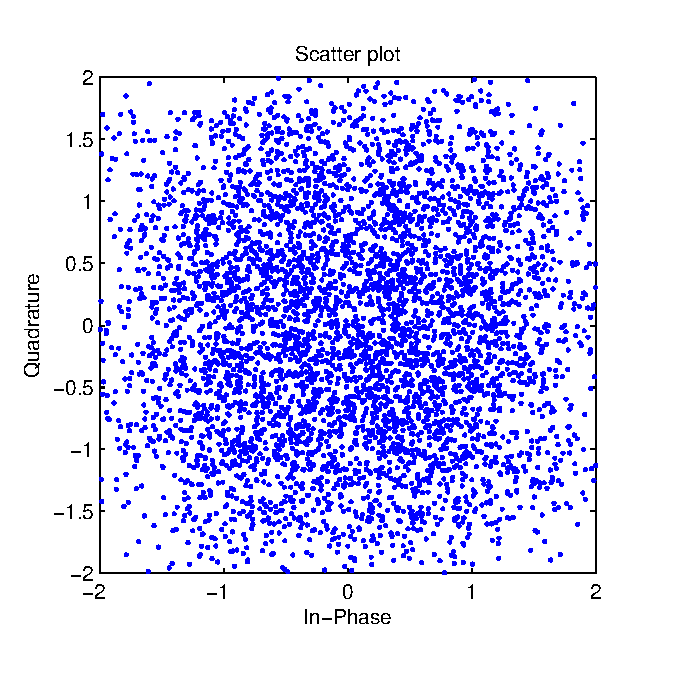
\includegraphics[width=1.2in]{71.eps}
\end{minipage}%
\begin{minipage}[t]{0.32\linewidth}
\centering
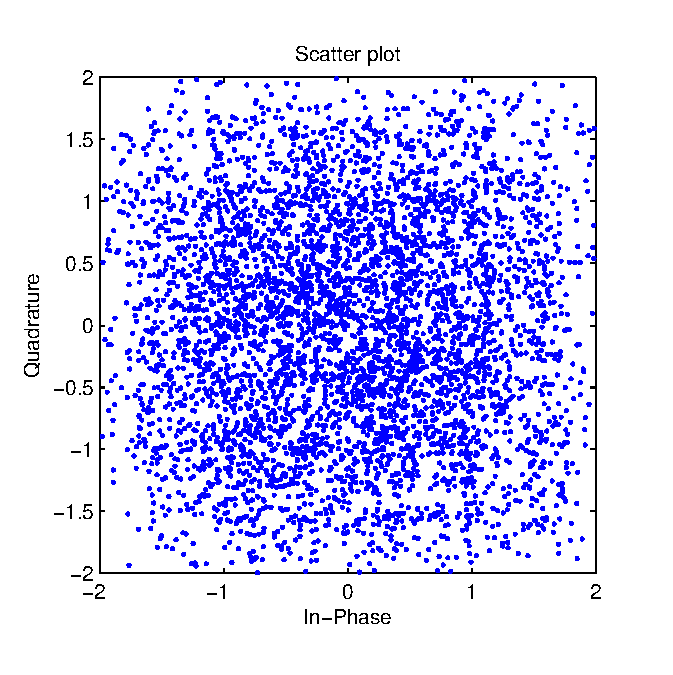
\includegraphics[width=1.2in]{72.eps}
\end{minipage}%
\begin{minipage}[t]{0.32\linewidth}
\centering
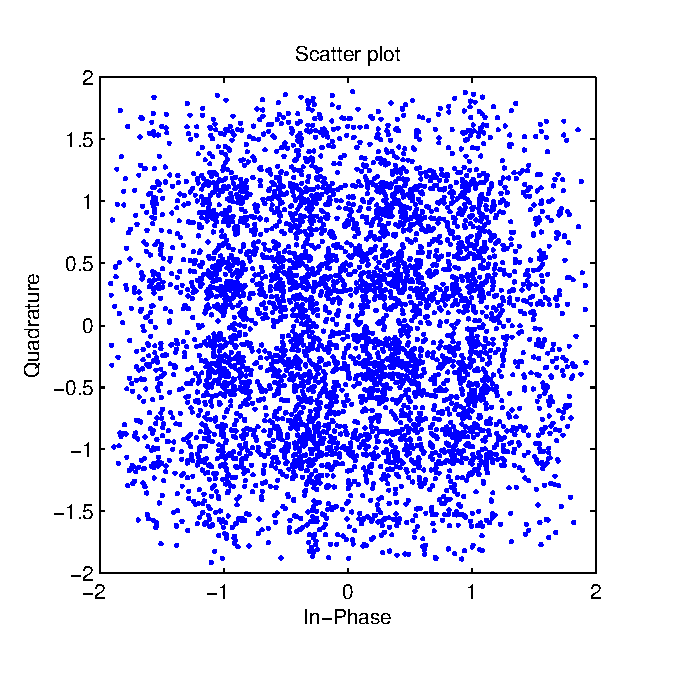
\includegraphics[width=1.2in]{75.eps}
\end{minipage}%
\end{figure}
